
\begin{frame}
  \frametitle{Training Set Database: Labels}
    \begin{block}{ORIGEN designations for reactor technologies and fuel assemblies:}
    \begin{table}
      \footnotesize
      \centering
      \begin{tabular}{@{}lll@{}}
      \toprule
        \textbf{PWR} & \textbf{BWR}  & \textbf{PHWR} \\ \toprule
        CE14x14      & GE7x7-0       & CANDU19       \\
        W17x17       & Abb8x8-1      & CANDU28       \\
        S18x18       & Atrium10x10-9 & CANDU37       \\
        BW15x15      & SVEA64-1      &               \\
        VVER440      &               &               \\
        VVER1000     &               &               \\ \bottomrule
      \end{tabular}
    \end{table}
    \end{block}
    \vspace{-10pt}
    \begin{block}{Simulation parameters for ORIGEN input files:}
    \begin{table}
      \footnotesize
      \centering
      \begin{tabular}{@{}llll@{}}
        \toprule
        & \textbf{PWR}              & \textbf{BWR}              & \textbf{PHWR} \\  \toprule
        Power Density [$MW/MTU$]                        
        & 25, 35, 41                & 10, 22                    & 2.2, 18, 22   \\
        \boxalert{Burnup} [$GWd/MTU$]                   
        & 2--68                     & 1--68                     & 0.45--12.6    \\
        Moderator Density [$g/cm^3$]                    
        & 0.71                      & \{0.1, 0.3, 0.5, 0.7\}    & 0.84          \\
        \boxalert{Enrichment} [$\%\:{}^{235}{\text{U}}$]
        & \{0.5, 1.5, 2, 3, 4, 5\}  & \{0.5, 1.5, 2, 3, 4, 5\}  & 0.711         \\
        \boxalert{Cooling Time} [$days$]                
        & \multicolumn{3}{c}{\{0--6000\} in 100-day steps}                      \\ \bottomrule
      \end{tabular}
    \end{table}
    \end{block}
\end{frame}


\begin{frame}
  \frametitle{Training Set Database: Labels}
  \begin{figure}
    \centering
      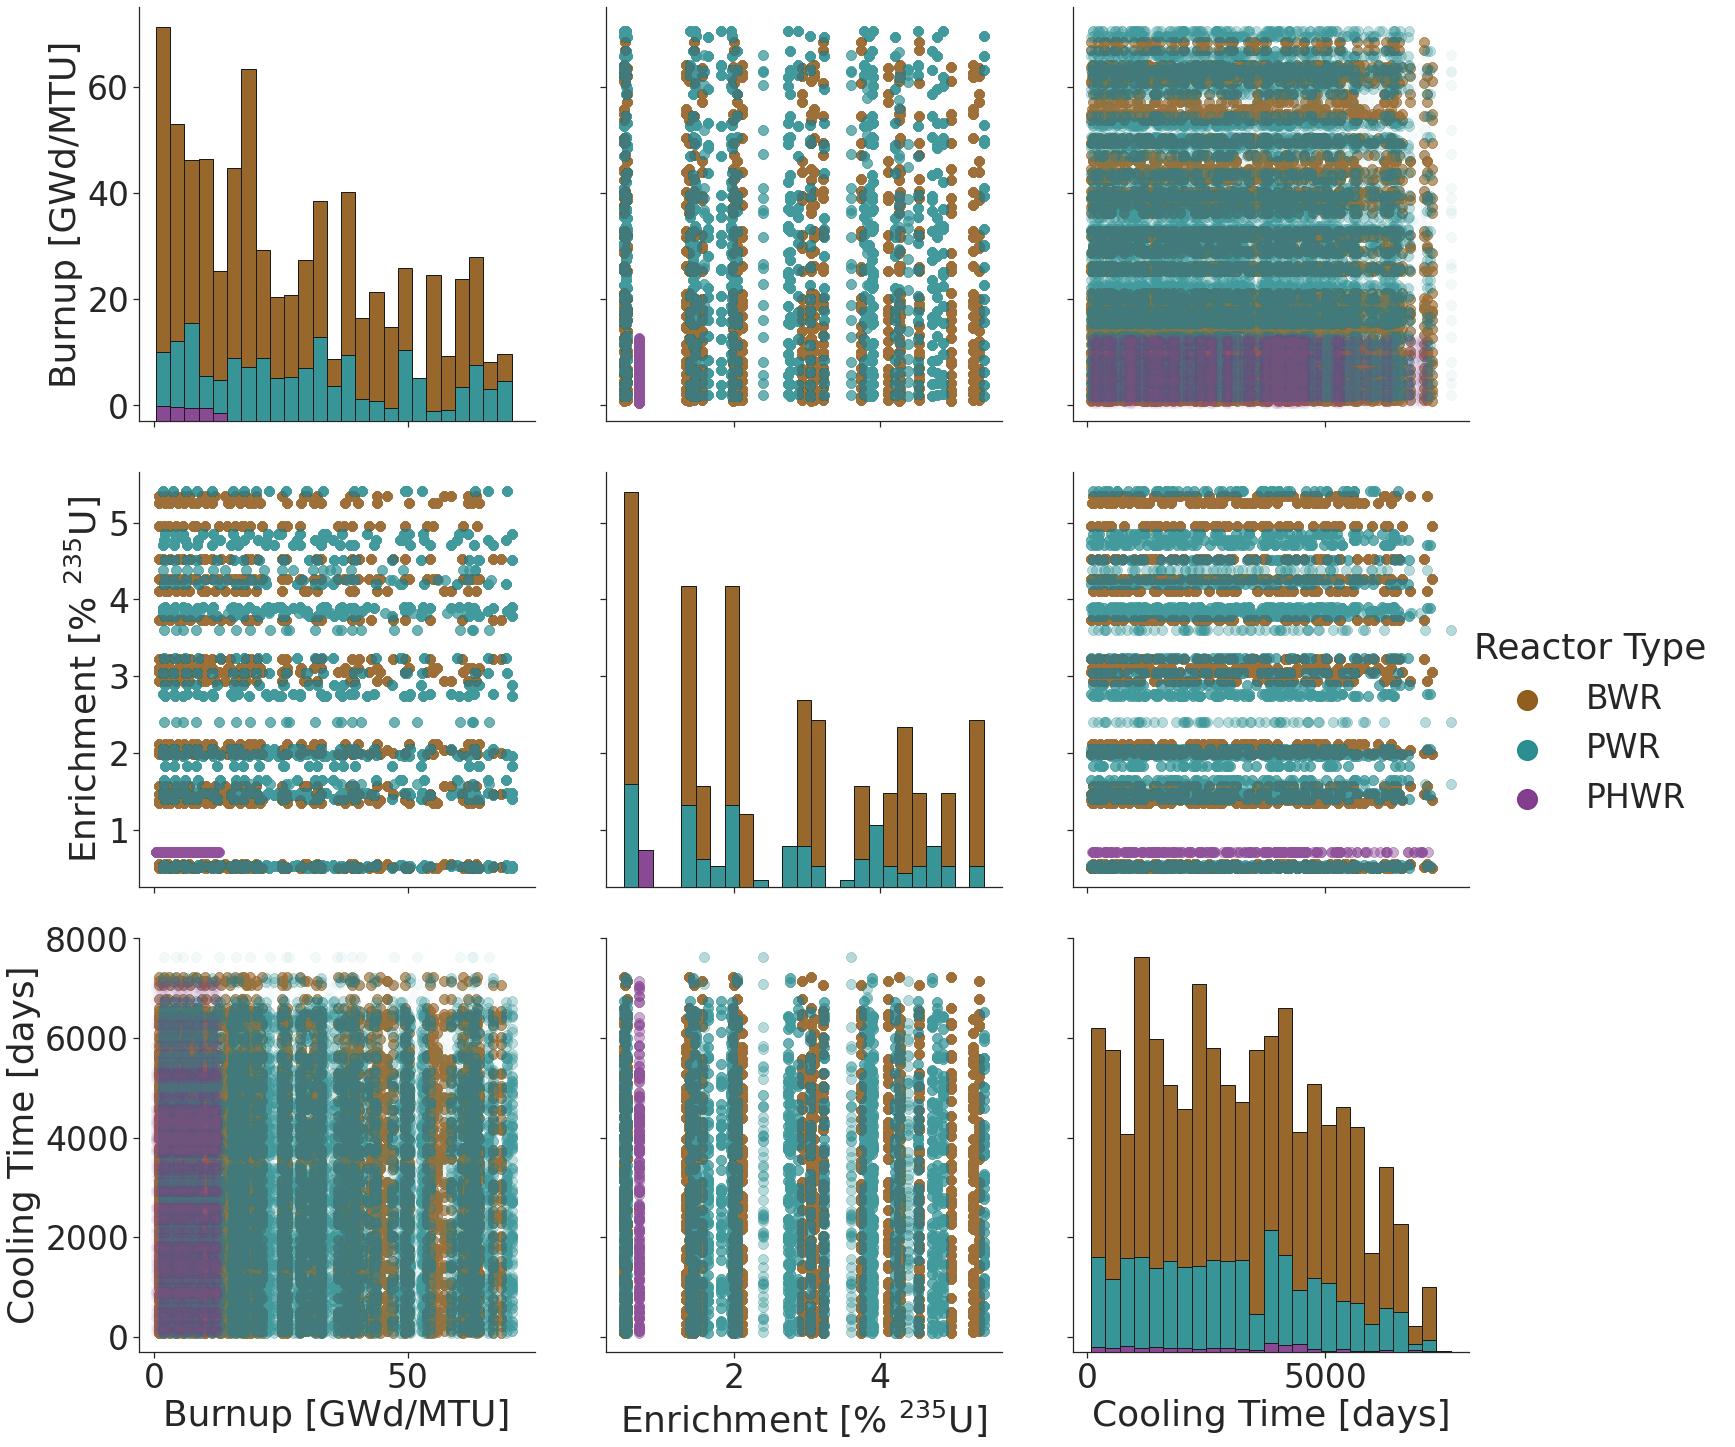
\includegraphics[height=0.85\textheight]{./figures/histogram_scatter_trainset_viz.png}
  \end{figure}
\end{frame}

\begin{frame}
  \frametitle{Training Set Database: Features}
    \begin{block}{Nuclide masses saved from ORIGEN simulations:}
    \begin{table}
      %\small
      \centering
      \renewcommand{\arraystretch}{1.3}
      \begin{tabular}{@{}|l|l|l|l|l|l|l|l|@{}}
        \hline
        \allbold{${}^{241}\text{Am}$} & ${}^{242m}\text{Am}$ &
        \allbold{${}^{243}\text{Am}$} & ${}^{242}\text{Cm}$ &
        \allbold{${}^{244}\text{Cm}$} & \allbold{${}^{134}\text{Cs}$} &
        \allbold{${}^{137}\text{Cs}$} & \allbold{${}^{154}\text{Eu}$} \\  
        \hline
        ${}^{143}\text{Nd}$ & ${}^{144}\text{Nd}$ & ${}^{145}\text{Nd}$ &
        ${}^{146}\text{Nd}$ & ${}^{148}\text{Nd}$ & ${}^{150}\text{Nd}$ &
        \allbold{${}^{237}\text{Np}$} & \allbold{${}^{238}\text{Pu}$} \\ 
        \hline
        \allbold{${}^{239}\text{Pu}$} & \allbold{${}^{240}\text{Pu}$} &
        ${}^{241}\text{Pu}$ & ${}^{242}\text{Pu}$ & ${}^{147}\text{Sm}$ &
        ${}^{149}\text{Sm}$ & ${}^{150}\text{Sm}$ & ${}^{151}\text{Sm}$ \\ 
        \hline
        ${}^{152}\text{Sm}$ & \allbold{${}^{234}\text{U}$} &
        \allbold{${}^{235}\text{U}$} & ${}^{236}\text{U}$ & ${}^{238}\text{U}$ &  &
        & \\  
        \hline
      \end{tabular}
    \end{table}
    \end{block}
    \begin{block}{Nuclide activities saved from ORIGEN simulations:}
    \begin{table}
      %\small
      \centering
      \renewcommand{\arraystretch}{1.3}
      \begin{tabular}{@{}|l|l|l|l|l|l|l|l|@{}}
        \hline
        ${}^{227}\text{Ac}$ & \allbold{${}^{241}\text{Am}$} &
        \allbold{${}^{243}\text{Am}$} & ${}^{133}\text{Ba}$ & ${}^{249}\text{Cf}$ &
        ${}^{252}\text{Cf}$ & ${}^{243}\text{Cm}$ & \allbold{${}^{244}\text{Cm}$} \\ 
        \hline
        ${}^{245}\text{Cm}$ & \allbold{${}^{134}\text{Cs}$} &
        \allbold{${}^{137}\text{Cs}$} & ${}^{152}\text{Eu}$ &
        \allbold{${}^{154}\text{Eu}$} & ${}^{166m}\text{Ho}$ & ${}^{85}\text{Kr}$ &
        ${}^{94}\text{Nb}$ \\ 
        \hline
        ${}^{236}\text{Np}$ & \allbold{${}^{237}\text{Np}$} & ${}^{231}\text{Pa}$ &
        ${}^{146}\text{Pm}$ & ${}^{236}\text{Pu}$ & \allbold{${}^{238}\text{Pu}$} &
        \allbold{${}^{239}\text{Pu}$} & \allbold{${}^{240}\text{Pu}$} \\ 
        \hline
        ${}^{226}\text{Ra}$ & ${}^{125}\text{Sb}$ & ${}^{228}\text{Th}$ &
        ${}^{229}\text{Th}$ & ${}^{232}\text{U}$  & ${}^{233}\text{U}$ &
        \allbold{${}^{234}\text{U}$}  & \allbold{${}^{235}\text{U}$}  \\ 
        \hline
      \end{tabular}
    \end{table}
    \end{block}
\end{frame}

\begin{frame}
  \frametitle{Information Reduction: Random \& Uniform Error}
  \begin{block}{Scikit-learn Algorithms}
    \small
    Introduced $0\% < E_{max} < 20\%$ random error:
    \[E_{max} = \text{0, 1, 2, 5, 8, 10, 12, 15, 18, 20}\% \]
    Each nuclide measurement is altered by a random percentage in the range: 
    \[[100-E_{max},100+E_{max}]\]
  \end{block}
  \begin{block}{Maximum Likelihood Calculations}
  \small
    Introduced uniform simulation uncertainty: 
    \[\sigma_i = \text{1, 5, 10, 15, 20}\% \]
    Each nuclide measurement is given a standard deviation via 
    \cite{mll_sensitivity}:
    \[\sigma_{Log L}^2 = \sum_i \left( 
                                \frac{x_{i,test} - x_{i,train}}{\sigma_{i,train}^2}
                                \right)^2 
                                (\sigma_{i,train}^2 + \sigma_{i,test}^2)
    \]
  \end{block}
\end{frame}

\begin{frame}
  \frametitle{Information Reduction: Processed Gamma Spectra}
  \begin{enumerate}
    \item Computational gamma detection 
    \item Process spectra: choose energy windows / window size
    \item Apply statistical counting error ($\sqrt{n}$) (using methods on previous slide)
  \end{enumerate}
  \begin{table}
    \small
    \centering
    \begin{tabular}{@{}lcllll@{}}
    \toprule
      \textbf{Detector} &
      \textbf{\begin{tabular}[c]{@{}c@{}}\% FWHM \\ @ 661 keV\end{tabular}} &
      \textbf{\begin{tabular}[c]{@{}l@{}}Distance \\ (cm)\end{tabular}} &
      \textbf{\begin{tabular}[c]{@{}l@{}}Height \\ (cm)\end{tabular}} &
      \textbf{\begin{tabular}[c]{@{}l@{}}Live Time\\ (s)\end{tabular}} &
      \textbf{\begin{tabular}[c]{@{}l@{}}Num \\ Channels\end{tabular}} \\ \midrule
      In-Lab HPGe           & 0.21 & 100.0 & 84.0  & 600  & 8192 \\
      Portable HPGe         & 0.29 & 100.0 & 100.0 & 600  & 8192 \\
      CZT                   & 1.20 & 100.0 & 100.0 & 600  & 1024 \\
      SrI\textsubscript{2}  & 2.94 & 100.0 & 100.0 & 600  & 1024 \\
      LaBr\textsubscript{3} & 3.63 & 213.0 & 84.5  & 2400 & 1024 \\
      NaI                   & 7.74 & 213.0 & 85.4  & 2400 & 1024 \\ \bottomrule
    \end{tabular}
  \end{table}
\end{frame}

\begin{frame}
  \frametitle{Gamma Spectra Processing}
  \begin{figure}
    \centering
    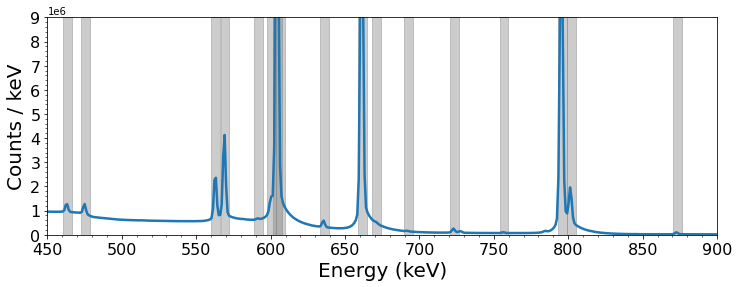
\includegraphics[width=\textwidth]{./figures/energy_window_example.png}
  \end{figure}
\end{frame}

\begin{frame}
  \frametitle{Gamma Spectra Processing}
  \begin{table}
    \small
    \centering
    \begin{tabular}{@{}lcm{0.5in}m{0.5in}m{0.5in}@{}}
      \toprule
      \multirow{2}{*}{\textbf{Detector}} &
      \multirow{2}{*}{\textbf{\begin{tabular}[c]{@{}l@{}}Energy Window\\ Size {[keV]}\end{tabular}}} &
      \multicolumn{3}{c}{\textbf{\# of Energy Windows}} \\ \cmidrule(l){3-5}
                       &    & Auto & Short & Long \\
      \toprule
      In-Lab HPGe      & 2  & 206  & 42    & 151  \\
      Portable HPGe    & 3  & 120  & 42    & 151  \\
      CZT              & 8  & 30   & 42    & 151  \\
      $\text{SrI}_2$   & 10 & 17   & 42    & 151  \\
      $\text{LaBr}_3$  & 12 & 19   & 42    & 151  \\
      NaI              & 12 & 9    & 42    & 151  \\ 
      \bottomrule
    \end{tabular}
  \end{table}
  \begin{table}
    \centering
    \renewcommand{\arraystretch}{1.3}
    \begin{tabular}{@{}|l|l|l|@{}}
      \hline
      \allbold{${}^{241}\text{Am}$} & \allbold{${}^{243}\text{Am}$} & ${}^{243}\text{Cm}$           \\ \hline
      ${}^{244}\text{Cm}$           & ${}^{245}\text{Cm}$           & \allbold{${}^{134}\text{Cs}$} \\ \hline
      \allbold{${}^{137}\text{Cs}$} & ${}^{152}\text{Eu}$           & \allbold{${}^{154}\text{Eu}$} \\ \hline
      \allbold{${}^{85}\text{Kr}$}  & ${}^{238}\text{Pu}$           & \allbold{${}^{125}\text{Sb}$} \\ \hline
    \end{tabular}
  \end{table}
\end{frame}

